\chapter{Elettrostatica}

\section{Legge di Coulomb}
  
La forza $\vec{F}_{12}$ esercitata da $q_1$ su $q_2$ è uguale in modulo e opposta in direzione alla forza $\vec{F}_{21}$ esercitata da $q_2$ su $q_1$.
    \begin{displaymath}
    	|\vec{F}_{12}| = |\vec{F}_{21}| = k_e \cdot \frac{q_1 \cdot q_2}{r^2}
    \end{displaymath}
Nel caso in cui le due cariche abbiano lo stesso segno:
	\begin{figure}[h!]
      \centering
      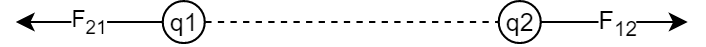
\includegraphics[scale=0.4]{Pictures/esempio1}
  \end{figure}
  	\begin{displaymath}\begin{aligned}
    	\vec{F}_{12} = - k_e \cdot \frac{q_1 \cdot q_2}{r^2} \cdot \vec{u}_r\\
        \vec{F}_{21} = k_e \cdot \frac{q_1 \cdot q_2}{r^2} \cdot \vec{u}_r
    \end{aligned}\end{displaymath}
Nel caso in cui le due cariche abbiano segno opposto:
    \begin{figure}[h!]
    	\centering
        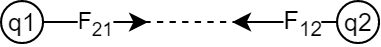
\includegraphics[scale=0.4]{Pictures/esempio2.png}
	\end{figure}
    \begin{displaymath}\begin{aligned}
        \vec{F}_{12} = k_e \cdot \frac{q_1 \cdot q_2}{r^2} \cdot \vec{u}_r\\
        \vec{F}_{21} = - k_e \cdot \frac{q_1 \cdot q_2}{r^2} \cdot \vec{u}_r
    \end{aligned}\end{displaymath}
    
\section{Principio di sovrapposizione}
In un sistema di $n$ cariche, volendo valutare la forza totale agente su una carica $q$, è necessario sommare le forze esercitate da ciascuna carica. Ciascuna di queste forze agisce come se fosse l'unica presente.
	\begin{displaymath}\begin{aligned}
		\vec{F} = \sum_{i=1}^n k_e \cdot \frac{q \cdot q_i}{r_i^2} \cdot \vec{u}_{r_i}
	\end{aligned}\end{displaymath}

\section{Campo elettrico}
Dato un sistema di $n$ cariche, su una carica di prova $q$, agisce un campo elettrico $\vec{E}$ dato da:
	\begin{displaymath}\begin{aligned}
		\vec{E} = \sum_{i=0}^n k_e \cdot \frac{q_i}{r_i^2}\vec{u}_{r_i}
	\end{aligned}\end{displaymath}
La forza agente su $q$ può essere espressa come:
	\begin{displaymath}
		\vec{F} = q \cdot \vec{E}
	\end{displaymath}
    
\section{Teorema di Gauss per il campo elettrico}
Il teorema di Gauss per il campo elettrico permette di calcolare il flusso del campo elettrico generato da una certa distribuzione di carica elettrica attraverso una superficie senza svolgere i calcoli prescritti dalla definizione di flusso.
Data una superficie chiusa $S$ contenente $n$ cariche elettriche (positive o negative), il flusso del campo elettrico (generato dalle cariche) attraverso tale superficie è uguale al rapporto tra carica totale contenuta nella superficie chiusa e la costante dielettrica $\epsilon$ del mezzo in cui si trovano le cariche ($\epsilon_0$ nel vuoto):
\begin{displaymath}
	\Phi_S(\vec{E}) = \frac{\sum_{i=1}^n q_i}{\epsilon_0}
\end{displaymath}

\subsection{Distribuzione lineare}
    \begin{figure}[h!]
    	\centering
    	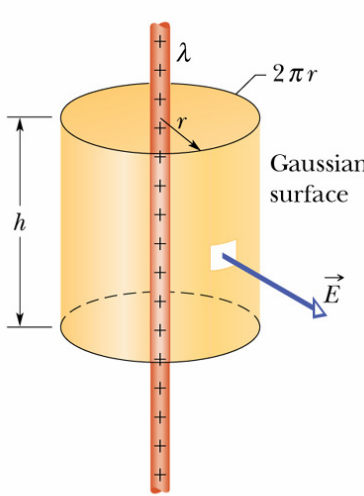
\includegraphics[scale=0.4]{Pictures/esempio3.png}
    \end{figure}
Il campo elettrico $\vec{E}$ è perpendicolare alla superficie gaussiana:
	\begin{itemize}
    	\item{$\Phi(\vec{E})$ attraverso le basi è nullo.}
        \item{$\Phi(\vec{E})$ attraverso la superficie laterale è pari a $E \cdot (2 \cdot \pi \cdot r \cdot h)$.}
    \end{itemize}
Per il teorema di Gauss:
	\begin{displaymath}\begin{aligned}
		\epsilon_0 \cdot \Phi(\vec{E}) = q\\
        \epsilon_0 \cdot \int_S \vec{E} \cdot d\vec{A} = q\\
        \epsilon_0 \cdot E \cdot (2 \cdot \pi \cdot r \cdot h) = q = \lambda \cdot h\\
        \vec{E} = \frac{\lambda}{2 \cdot \epsilon_0 \cdot \pi \cdot r \cdot h}
	\end{aligned}\end{displaymath}
  
\subsection{Distribuzione piana}
    \begin{figure}[h!]
    	\centering
    	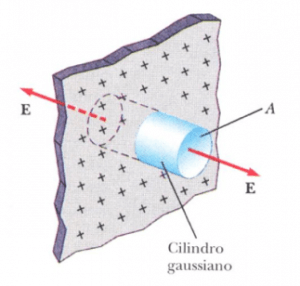
\includegraphics[scale=0.4]{Pictures/esempio4.png}
    \end{figure}
Il campo elettrico $\vec{E}$ è perpendicolare alla superficie gaussiana:
	\begin{itemize}
    	\item{$\Phi(\vec{E})$ attraverso la superficie del cilindro è nullo.}
        \item{$\Phi(\vec{E})$ attraverso la le basi del cilindro è pari a $E \cdot A$, dove $A$ è l'area di una base.}
    \end{itemize}
Per il teorema di Gauss:
	\begin{displaymath}\begin{aligned}
		\epsilon_0 \cdot \Phi(\vec{E}) = q\\
        \epsilon_0 \cdot \int_S \vec{E} \cdot d\vec{A} = q\\
        \epsilon_0 \cdot (E\cdot A + E \cdot A) = q \cdot \sigma \cdot A\\
        2 \cdot \epsilon_0 \cdot E\cdot A = q = \sigma \cdot A\\
        E = \frac{\sigma}{2 \epsilon_0}
	\end{aligned}\end{displaymath}


\section{Energia elettrica}
\subsection{Energia potenziale elettrica}
L'energia potenziale è l'inverso del lavoro compiuto dalla forza per spostare $q_2$ dal punto $A$ al punto $B$.
	\begin{displaymath}\begin{aligned}
		\Delta U = - \int_A^B \vec{F} \cdot d\vec{s} = \\
        = - \int_A^B \vec{F} \cdot d\vec{r} = -\int_{r_A}^{r_B} k_e \cdot \frac{q_1 \cdot q_2}{r^2} dr =\\
        = k_e\cdot q_1 \cdot q_2 \cdot  \left(\frac{1}{r_B} - \frac{1}{r_A}\right)
	\end{aligned}\end{displaymath}

\subsection{Potenziale elettrico}
Sia $q_0$ una carica di prova in moto da $A$ a $B$, sotto l'azione di un campo elettrico $\vec{E}$:
	\begin{displaymath}
		\Delta V= \frac{\Delta U}{q_0} = \frac{-L_{AB}}{q_0} \qquad V = \frac{U}{q_0}
	\end{displaymath}

\subsection{Lavoro del campo elettrico}
Il lavoro compiuto dal campo elettrico per spostare una particella $q_0$ da $A$ a $B$:
\begin{displaymath}
	L_{AB} = q_0 \cdot (-\Delta V)		
\end{displaymath}


\subsection{La forza di Coulomb è conservativa}
Una forza è conservativa quando il lavoro da essa compiuto può essere scritto come una differenza di potenziale:
\begin{displaymath}\begin{aligned}
	L_{AB} = \int_A^B \vec{F} \cdot d\vec{r} = \int_A^B k_e \cdot \frac{q_1q_2}{r^2} \cdot \vec{u}_r \cdot d\vec{r} =\\
    = k_e \cdot q_1q_2 \cdot \int_A^B \frac{1}{r^2} = \left( k_e \frac{q_1q_2}{r_B}\right) - \left(k_e\frac{q_1q_2}{r_A}\right) = U(B) - U(A)
\end{aligned}\end{displaymath}
Questo risultato significa che:
\begin{itemize}
	\item{Il lavoro lungo un percorso chiuso è nullo.}
    \item{Il lavoro lungo uno spostamento dipende solo dal punto di partenza e dal punto di arrivo e non dal percorso seguito.}
\end{itemize}

\section{Dipolo elettrico}
Un dipolo elettrico è un sistema composto da due cariche uguali, di segno opposto, poste a distanza $d$ lungo un asse $u_x$.\\
\begin{figure}[h!]
	\centering
    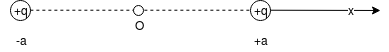
\includegraphics[scale=0.6]{Pictures/DipoloElettrico}
\end{figure}
Viene definito il \textbf{momento di dipolo} $\vec{p}$ come 
\begin{displaymath}
	\vec{p} = q \cdot d \cdot \vec{u}_x
\end{displaymath}

\subsection{Campo elettrico lungo l'asse del dipolo}
\begin{displaymath}\begin{aligned}
	\vec{E}_+ = k_e \cdot \frac{q}{(r_x - a)^2} \cdot \vec{i}\\
    \vec{E}_- = - k_e \cdot \frac{q}{(r_x + a)^2} \cdot \vec{i}\\\\
    \vec{E} = k_e \cdot \left(\frac{q}{(r_x - a)^2} - \frac{q}{(r_x^2 + a^2)^2} \right) \cdot \vec{i} = \\
    = k_e \cdot q \left( \frac{(r_x + a)^2 - (r_x - a)^2}{(r_x^2 + a^2)^2} \right) \cdot \vec{i} = \\
    = k_e \cdot q \frac{r_x^2 + a^2 + 2 r_x a - r_x^2 +2 r_x a - a^2}{(r_x^2 + a^2)^2} \cdot \vec{i} = 
    = k_e \cdot \frac{4 q r_x a}{(r_x^2 + a^2)^2} \cdot \vec{i}
\end{aligned}\end{displaymath}
Ricordando che $a = \frac{d}{2}$ e che $p = qd$:
\begin{displaymath}\begin{aligned}
	\vec{E} = k_e \cdot \frac{2p\cdot r_x}{(r_x^2 + \frac{d}{2}^2)^2} \cdot \vec{i}    
\end{aligned}\end{displaymath}
Ha senso, in applicazioni reali considerare $r_x >>> d$, cioè misurare il campo elettrico a distanze molto maggiori della distanza tra le cariche del dipolo.
\begin{displaymath}
\vec{E} = k_e \cdot \frac{2 p r_x}{r_x^4} \cdot \vec{i} = k_e \cdot \frac{2p}{r_x^3} \cdot \vec{i}
\end{displaymath}

\subsection{Potenziale elettrico lungo l'asse del dipolo}
Il potenziale generato da una carica a una distanza $r$ è dato da:
\begin{displaymath}
	V(r) = k_e \cdot \frac{q}{r}
\end{displaymath}
Perciò, il potenziale del dipolo a una distanza $r_x$ è dato da:
\begin{displaymath}\begin{aligned}
	V(r_x) = k_e \cdot \left( \frac{q}{r_x-a} - \frac{q}{r_x+a} \right) =\\ 
    k_e \cdot q \left( \frac{r_x + a - r_x + a}{r_x^2 -a^2} \right)=\\
    k_e \cdot q \cdot \frac{2a}{r_x^2-a^2}
\end{aligned}\end{displaymath}
Ricordando che $a = \frac{d}{2}$ e che $p = qd$:
\begin{displaymath}\begin{aligned}
	\vec{V} = k_e \cdot \frac{p}{r_x^2 - \frac{d}{2}^2}    
\end{aligned}\end{displaymath}
Ha senso, in applicazioni reali considerare $r_x >>> d$, cioè misurare il potenziale a distanze molto maggiori della distanza tra le cariche del dipolo.
\begin{displaymath}
	\vec{V} = k_e \cdot \frac{p}{r_x^2}
\end{displaymath}
